\documentclass[twoside]{book}

% Packages required by doxygen
\usepackage{fixltx2e}
\usepackage{calc}
\usepackage{doxygen}
\usepackage[export]{adjustbox} % also loads graphicx
\usepackage{graphicx}
\usepackage[utf8]{inputenc}
\usepackage{makeidx}
\usepackage{multicol}
\usepackage{multirow}
\PassOptionsToPackage{warn}{textcomp}
\usepackage{textcomp}
\usepackage[nointegrals]{wasysym}
\usepackage[table]{xcolor}

% Font selection
\usepackage[T1]{fontenc}
\usepackage[scaled=.90]{helvet}
\usepackage{courier}
\usepackage{amssymb}
\usepackage{sectsty}
\renewcommand{\familydefault}{\sfdefault}
\allsectionsfont{%
  \fontseries{bc}\selectfont%
  \color{darkgray}%
}
\renewcommand{\DoxyLabelFont}{%
  \fontseries{bc}\selectfont%
  \color{darkgray}%
}
\newcommand{\+}{\discretionary{\mbox{\scriptsize$\hookleftarrow$}}{}{}}

% Page & text layout
\usepackage{geometry}
\geometry{%
  a4paper,%
  top=2.5cm,%
  bottom=2.5cm,%
  left=2.5cm,%
  right=2.5cm%
}
\tolerance=750
\hfuzz=15pt
\hbadness=750
\setlength{\emergencystretch}{15pt}
\setlength{\parindent}{0cm}
\setlength{\parskip}{3ex plus 2ex minus 2ex}
\makeatletter
\renewcommand{\paragraph}{%
  \@startsection{paragraph}{4}{0ex}{-1.0ex}{1.0ex}{%
    \normalfont\normalsize\bfseries\SS@parafont%
  }%
}
\renewcommand{\subparagraph}{%
  \@startsection{subparagraph}{5}{0ex}{-1.0ex}{1.0ex}{%
    \normalfont\normalsize\bfseries\SS@subparafont%
  }%
}
\makeatother

% Headers & footers
\usepackage{fancyhdr}
\pagestyle{fancyplain}
\fancyhead[LE]{\fancyplain{}{\bfseries\thepage}}
\fancyhead[CE]{\fancyplain{}{}}
\fancyhead[RE]{\fancyplain{}{\bfseries\leftmark}}
\fancyhead[LO]{\fancyplain{}{\bfseries\rightmark}}
\fancyhead[CO]{\fancyplain{}{}}
\fancyhead[RO]{\fancyplain{}{\bfseries\thepage}}
\fancyfoot[LE]{\fancyplain{}{}}
\fancyfoot[CE]{\fancyplain{}{}}
\fancyfoot[RE]{\fancyplain{}{\bfseries\scriptsize Generated by Doxygen }}
\fancyfoot[LO]{\fancyplain{}{\bfseries\scriptsize Generated by Doxygen }}
\fancyfoot[CO]{\fancyplain{}{}}
\fancyfoot[RO]{\fancyplain{}{}}
\renewcommand{\footrulewidth}{0.4pt}
\renewcommand{\chaptermark}[1]{%
  \markboth{#1}{}%
}
\renewcommand{\sectionmark}[1]{%
  \markright{\thesection\ #1}%
}

% Indices & bibliography
\usepackage{natbib}
\usepackage[titles]{tocloft}
\setcounter{tocdepth}{3}
\setcounter{secnumdepth}{5}
\makeindex

% Hyperlinks (required, but should be loaded last)
\usepackage{ifpdf}
\ifpdf
  \usepackage[pdftex,pagebackref=true]{hyperref}
\else
  \usepackage[ps2pdf,pagebackref=true]{hyperref}
\fi
\hypersetup{%
  colorlinks=true,%
  linkcolor=blue,%
  citecolor=blue,%
  unicode%
}

% Custom commands
\newcommand{\clearemptydoublepage}{%
  \newpage{\pagestyle{empty}\cleardoublepage}%
}

\usepackage{caption}
\captionsetup{labelsep=space,justification=centering,font={bf},singlelinecheck=off,skip=4pt,position=top}

%===== C O N T E N T S =====

\begin{document}

% Titlepage & ToC
\hypersetup{pageanchor=false,
             bookmarksnumbered=true,
             pdfencoding=unicode
            }
\pagenumbering{alph}
\begin{titlepage}
\vspace*{7cm}
\begin{center}%
{\Large My Project }\\
\vspace*{1cm}
{\large Generated by Doxygen 1.8.14}\\
\end{center}
\end{titlepage}
\clearemptydoublepage
\pagenumbering{roman}
\tableofcontents
\clearemptydoublepage
\pagenumbering{arabic}
\hypersetup{pageanchor=true}

%--- Begin generated contents ---
\chapter{R\+E\+A\+D\+ME}
\label{md__r_e_a_d_m_e}
\Hypertarget{md__r_e_a_d_m_e}
Hannes project

\href{https://gitlab.mpikg.mpg.de/baukmann/hannesProjekt/blob/master/html/index.html}{\tt Documentation} 
\chapter{Namespace Index}
\section{Namespace List}
Here is a list of all documented namespaces with brief descriptions\+:\begin{DoxyCompactList}
\item\contentsline{section}{\mbox{\hyperlink{namespace_hannes_o_o_p_project}{Hannes\+O\+O\+P\+Project}} \\*Description of this project }{\pageref{namespace_hannes_o_o_p_project}}{}
\end{DoxyCompactList}

\chapter{Hierarchical Index}
\section{Class Hierarchy}
This inheritance list is sorted roughly, but not completely, alphabetically\+:\begin{DoxyCompactList}
\item \contentsline{section}{O\+O\+P.\+Analysis}{\pageref{class_o_o_p_1_1_analysis}}{}
\item \contentsline{section}{O\+O\+P\+\_\+np\+Array.\+Analysis}{\pageref{class_o_o_p__np_array_1_1_analysis}}{}
\item \contentsline{section}{O\+O\+P\+\_\+np\+Array.\+Builder}{\pageref{class_o_o_p__np_array_1_1_builder}}{}
\item \contentsline{section}{O\+O\+P.\+Builder}{\pageref{class_o_o_p_1_1_builder}}{}
\item \contentsline{section}{O\+O\+P\+\_\+np\+Array.\+Cytokine}{\pageref{class_o_o_p__np_array_1_1_cytokine}}{}
\item \contentsline{section}{O\+O\+P.\+Cytokine}{\pageref{class_o_o_p_1_1_cytokine}}{}
\item \contentsline{section}{O\+O\+P.\+Glycan}{\pageref{class_o_o_p_1_1_glycan}}{}
\item \contentsline{section}{O\+O\+P\+\_\+np\+Array.\+Glycan}{\pageref{class_o_o_p__np_array_1_1_glycan}}{}
\item \contentsline{section}{O\+O\+P.\+Lectin}{\pageref{class_o_o_p_1_1_lectin}}{}
\item \contentsline{section}{O\+O\+P\+\_\+np\+Array.\+Lectin}{\pageref{class_o_o_p__np_array_1_1_lectin}}{}
\item \contentsline{section}{O\+O\+P.\+Simulation}{\pageref{class_o_o_p_1_1_simulation}}{}
\item \contentsline{section}{O\+O\+P\+\_\+np\+Array.\+Simulation}{\pageref{class_o_o_p__np_array_1_1_simulation}}{}
\item \contentsline{section}{O\+O\+P.\+Sphere}{\pageref{class_o_o_p_1_1_sphere}}{}
\begin{DoxyCompactList}
\item \contentsline{section}{O\+O\+P.\+Bead}{\pageref{class_o_o_p_1_1_bead}}{}
\item \contentsline{section}{O\+O\+P.\+Decoder\+Cell}{\pageref{class_o_o_p_1_1_decoder_cell}}{}
\end{DoxyCompactList}
\item \contentsline{section}{O\+O\+P\+\_\+np\+Array.\+Sphere}{\pageref{class_o_o_p__np_array_1_1_sphere}}{}
\begin{DoxyCompactList}
\item \contentsline{section}{O\+O\+P\+\_\+np\+Array.\+Bead}{\pageref{class_o_o_p__np_array_1_1_bead}}{}
\item \contentsline{section}{O\+O\+P\+\_\+np\+Array.\+Decoder\+Cell}{\pageref{class_o_o_p__np_array_1_1_decoder_cell}}{}
\end{DoxyCompactList}
\item \contentsline{section}{O\+O\+P\+\_\+np\+Array.\+Well}{\pageref{class_o_o_p__np_array_1_1_well}}{}
\begin{DoxyCompactList}
\item \contentsline{section}{O\+O\+P\+\_\+np\+Array.\+Well\+\_\+list}{\pageref{class_o_o_p__np_array_1_1_well__list}}{}
\item \contentsline{section}{O\+O\+P\+\_\+np\+Array.\+Well\+\_\+np\+Array}{\pageref{class_o_o_p__np_array_1_1_well__np_array}}{}
\end{DoxyCompactList}
\item \contentsline{section}{O\+O\+P.\+Well}{\pageref{class_o_o_p_1_1_well}}{}
\end{DoxyCompactList}

\chapter{Class Index}
\section{Class List}
Here are the classes, structs, unions and interfaces with brief descriptions\+:\begin{DoxyCompactList}
\item\contentsline{section}{\mbox{\hyperlink{class_o_o_p_1_1_cell}{O\+O\+P.\+Cell}} \\*Dokumentation for class \mbox{\hyperlink{class_o_o_p_1_1_cell}{Cell}} }{\pageref{class_o_o_p_1_1_cell}}{}
\item\contentsline{section}{\mbox{\hyperlink{class_o_o_p_1_1_decoder_cell}{O\+O\+P.\+Decoder\+Cell}} }{\pageref{class_o_o_p_1_1_decoder_cell}}{}
\item\contentsline{section}{\mbox{\hyperlink{class_o_o_p_1_1_encoder_cell}{O\+O\+P.\+Encoder\+Cell}} }{\pageref{class_o_o_p_1_1_encoder_cell}}{}
\item\contentsline{section}{\mbox{\hyperlink{class_o_o_p_1_1_glycan}{O\+O\+P.\+Glycan}} }{\pageref{class_o_o_p_1_1_glycan}}{}
\item\contentsline{section}{\mbox{\hyperlink{class_o_o_p_1_1_lectin}{O\+O\+P.\+Lectin}} }{\pageref{class_o_o_p_1_1_lectin}}{}
\item\contentsline{section}{\mbox{\hyperlink{classprototype_1_1_object_factory}{prototype.\+Object\+Factory}} }{\pageref{classprototype_1_1_object_factory}}{}
\item\contentsline{section}{\mbox{\hyperlink{classprototype_1_1_prototype}{prototype.\+Prototype}} }{\pageref{classprototype_1_1_prototype}}{}
\item\contentsline{section}{\mbox{\hyperlink{classprototype_1_1_type1}{prototype.\+Type1}} }{\pageref{classprototype_1_1_type1}}{}
\item\contentsline{section}{\mbox{\hyperlink{classprototype_1_1_type2}{prototype.\+Type2}} }{\pageref{classprototype_1_1_type2}}{}
\end{DoxyCompactList}

\chapter{Namespace Documentation}
\hypertarget{namespace_hannes_o_o_p_project}{}\section{Hannes\+O\+O\+P\+Project Namespace Reference}
\label{namespace_hannes_o_o_p_project}\index{Hannes\+O\+O\+P\+Project@{Hannes\+O\+O\+P\+Project}}


Description of this project.  




\subsection{Detailed Description}
Description of this project. 

\subsection*{Ueberschift! }
\chapter{Class Documentation}
\hypertarget{class_o_o_p__np_array_1_1_analysis}{}\section{O\+O\+P\+\_\+np\+Array.\+Analysis Class Reference}
\label{class_o_o_p__np_array_1_1_analysis}\index{O\+O\+P\+\_\+np\+Array.\+Analysis@{O\+O\+P\+\_\+np\+Array.\+Analysis}}
\subsection*{Public Member Functions}
\begin{DoxyCompactItemize}
\item 
\mbox{\Hypertarget{class_o_o_p__np_array_1_1_analysis_a7a0c59492d240f1e2c12e5357b14d42a}\label{class_o_o_p__np_array_1_1_analysis_a7a0c59492d240f1e2c12e5357b14d42a}} 
def {\bfseries \+\_\+\+\_\+init\+\_\+\+\_\+} (self)
\item 
\mbox{\Hypertarget{class_o_o_p__np_array_1_1_analysis_a862e82b32a1059f7e85c6af2cafd92b3}\label{class_o_o_p__np_array_1_1_analysis_a862e82b32a1059f7e85c6af2cafd92b3}} 
def {\bfseries count\+Cytokines} (self, simulation\+Results)
\item 
\mbox{\Hypertarget{class_o_o_p__np_array_1_1_analysis_aed7eba5773c07b47d905869251898f62}\label{class_o_o_p__np_array_1_1_analysis_aed7eba5773c07b47d905869251898f62}} 
def {\bfseries plot\+Cytokines} (self, simulation\+Results)
\end{DoxyCompactItemize}
\subsection*{Public Attributes}
\begin{DoxyCompactItemize}
\item 
\mbox{\Hypertarget{class_o_o_p__np_array_1_1_analysis_a0d725e11b898861453a55b234617348d}\label{class_o_o_p__np_array_1_1_analysis_a0d725e11b898861453a55b234617348d}} 
{\bfseries cytokine\+Amount}
\item 
\mbox{\Hypertarget{class_o_o_p__np_array_1_1_analysis_a6617ebceb7332d29e18f1be6f72f38cb}\label{class_o_o_p__np_array_1_1_analysis_a6617ebceb7332d29e18f1be6f72f38cb}} 
{\bfseries cytokine\+Names}
\end{DoxyCompactItemize}


The documentation for this class was generated from the following file\+:\begin{DoxyCompactItemize}
\item 
O\+O\+P\+\_\+np\+Array.\+py\end{DoxyCompactItemize}

\hypertarget{class_o_o_p__np_array_1_1_bead}{}\section{O\+O\+P\+\_\+np\+Array.\+Bead Class Reference}
\label{class_o_o_p__np_array_1_1_bead}\index{O\+O\+P\+\_\+np\+Array.\+Bead@{O\+O\+P\+\_\+np\+Array.\+Bead}}


\mbox{\hyperlink{class_o_o_p__np_array_1_1_bead}{Bead}} is a subclass of \mbox{\hyperlink{class_o_o_p__np_array_1_1_sphere}{Sphere}} and represents beads (made of P\+M\+MA, or acrylic glass) loaded with glycan structures.  


Inheritance diagram for O\+O\+P\+\_\+np\+Array.\+Bead\+:\begin{figure}[H]
\begin{center}
\leavevmode
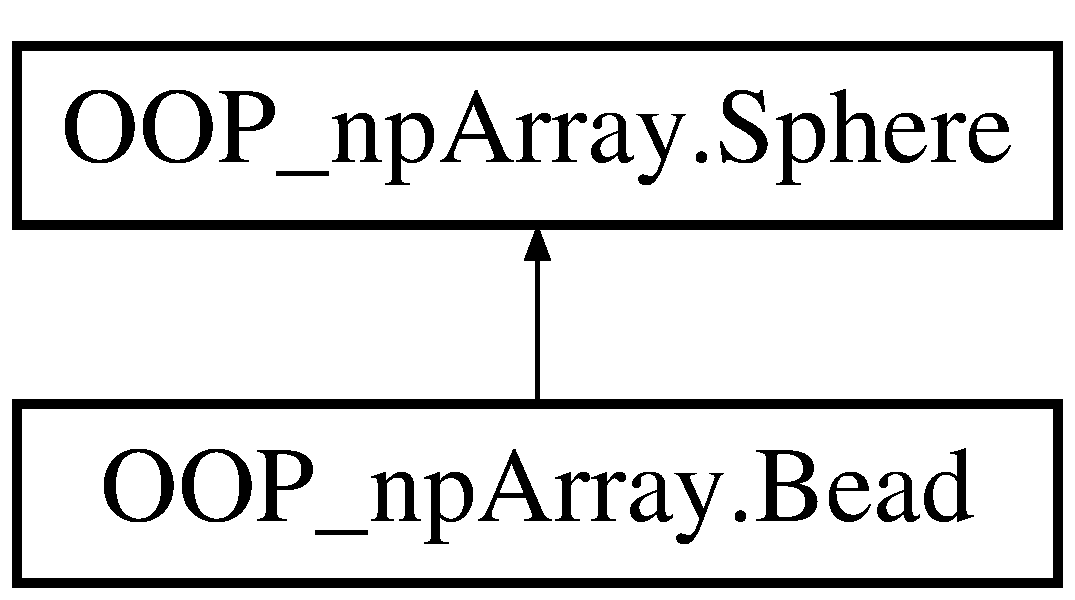
\includegraphics[height=2.000000cm]{class_o_o_p__np_array_1_1_bead}
\end{center}
\end{figure}
\subsection*{Public Member Functions}
\begin{DoxyCompactItemize}
\item 
\mbox{\Hypertarget{class_o_o_p__np_array_1_1_bead_a519936bf65fdbd556b6f48672140383b}\label{class_o_o_p__np_array_1_1_bead_a519936bf65fdbd556b6f48672140383b}} 
def {\bfseries \+\_\+\+\_\+init\+\_\+\+\_\+} (self, args)
\item 
def \mbox{\hyperlink{class_o_o_p__np_array_1_1_bead_a107832d8794984eb40de00557d1ddfcc}{attach\+Glycans}} (self, glycan\+\_\+names\+\_\+list, glycan\+\_\+types\+\_\+list, density\+\_\+percentage)
\begin{DoxyCompactList}\small\item\em Method to attach \mbox{\hyperlink{class_o_o_p__np_array_1_1_glycan}{Glycan}} objects to \mbox{\hyperlink{class_o_o_p__np_array_1_1_bead}{Bead}} objects. \end{DoxyCompactList}\end{DoxyCompactItemize}
\subsection*{Public Attributes}
\begin{DoxyCompactItemize}
\item 
\mbox{\Hypertarget{class_o_o_p__np_array_1_1_bead_a0ea948de6ab932e0d61acab9a1eec37b}\label{class_o_o_p__np_array_1_1_bead_a0ea948de6ab932e0d61acab9a1eec37b}} 
{\bfseries glycan\+\_\+density}
\item 
\mbox{\Hypertarget{class_o_o_p__np_array_1_1_bead_a37d48a1d59eabe3093c6f7452443b5a7}\label{class_o_o_p__np_array_1_1_bead_a37d48a1d59eabe3093c6f7452443b5a7}} 
{\bfseries glycan}
\end{DoxyCompactItemize}


\subsection{Detailed Description}
\mbox{\hyperlink{class_o_o_p__np_array_1_1_bead}{Bead}} is a subclass of \mbox{\hyperlink{class_o_o_p__np_array_1_1_sphere}{Sphere}} and represents beads (made of P\+M\+MA, or acrylic glass) loaded with glycan structures. 

\subsection{Member Function Documentation}
\mbox{\Hypertarget{class_o_o_p__np_array_1_1_bead_a107832d8794984eb40de00557d1ddfcc}\label{class_o_o_p__np_array_1_1_bead_a107832d8794984eb40de00557d1ddfcc}} 
\index{O\+O\+P\+\_\+np\+Array\+::\+Bead@{O\+O\+P\+\_\+np\+Array\+::\+Bead}!attach\+Glycans@{attach\+Glycans}}
\index{attach\+Glycans@{attach\+Glycans}!O\+O\+P\+\_\+np\+Array\+::\+Bead@{O\+O\+P\+\_\+np\+Array\+::\+Bead}}
\subsubsection{\texorpdfstring{attach\+Glycans()}{attachGlycans()}}
{\footnotesize\ttfamily def O\+O\+P\+\_\+np\+Array.\+Bead.\+attach\+Glycans (\begin{DoxyParamCaption}\item[{}]{self,  }\item[{}]{glycan\+\_\+names\+\_\+list,  }\item[{}]{glycan\+\_\+types\+\_\+list,  }\item[{}]{density\+\_\+percentage }\end{DoxyParamCaption})}



Method to attach \mbox{\hyperlink{class_o_o_p__np_array_1_1_glycan}{Glycan}} objects to \mbox{\hyperlink{class_o_o_p__np_array_1_1_bead}{Bead}} objects. 

Every \mbox{\hyperlink{class_o_o_p__np_array_1_1_bead}{Bead}} objects contains one type of \mbox{\hyperlink{class_o_o_p__np_array_1_1_glycan}{Glycan}} with a given density. Parameters glycan\+\_\+names\+\_\+list and glycan\+\_\+types\+\_\+list are handed over to the constructor of \mbox{\hyperlink{class_o_o_p__np_array_1_1_glycan}{Glycan}}.


\begin{DoxyParams}[1]{Parameters}
\mbox{\tt in}  & {\em glycan\+\_\+names\+\_\+list} & List of names of all Glycans to be added to the \mbox{\hyperlink{class_o_o_p__np_array_1_1_bead}{Bead}}. List may contain any number of member, including 0 \\
\hline
\mbox{\tt in}  & {\em see} & documentation for class \mbox{\hyperlink{class_o_o_p__np_array_1_1_glycan}{Glycan}}. \\
\hline
\mbox{\tt in}  & {\em see} & documentation for class \mbox{\hyperlink{class_o_o_p__np_array_1_1_glycan}{Glycan}}. \\
\hline
\end{DoxyParams}


The documentation for this class was generated from the following file\+:\begin{DoxyCompactItemize}
\item 
O\+O\+P\+\_\+np\+Array.\+py\end{DoxyCompactItemize}

\hypertarget{class_o_o_p__np_array_1_1_builder}{}\section{O\+O\+P\+\_\+np\+Array.\+Builder Class Reference}
\label{class_o_o_p__np_array_1_1_builder}\index{O\+O\+P\+\_\+np\+Array.\+Builder@{O\+O\+P\+\_\+np\+Array.\+Builder}}
\subsection*{Public Member Functions}
\begin{DoxyCompactItemize}
\item 
\mbox{\Hypertarget{class_o_o_p__np_array_1_1_builder_a50cbc2b655fea7a4d19ffc052186d235}\label{class_o_o_p__np_array_1_1_builder_a50cbc2b655fea7a4d19ffc052186d235}} 
def {\bfseries \+\_\+\+\_\+init\+\_\+\+\_\+} (self, x, y, z)
\item 
\mbox{\Hypertarget{class_o_o_p__np_array_1_1_builder_a3a5e9094d0a146909bee2801e6eaa2a6}\label{class_o_o_p__np_array_1_1_builder_a3a5e9094d0a146909bee2801e6eaa2a6}} 
def {\bfseries build\+Well} (self, container\+\_\+type, n\+\_\+beads, n\+\_\+cells)
\item 
\mbox{\Hypertarget{class_o_o_p__np_array_1_1_builder_a16432a43a2c78f298da41e298034092c}\label{class_o_o_p__np_array_1_1_builder_a16432a43a2c78f298da41e298034092c}} 
def {\bfseries build\+Bead} (self, i, ID, glyan\+\_\+name\+\_\+string, glycan\+\_\+type\+\_\+string, density\+\_\+percentage)
\item 
\mbox{\Hypertarget{class_o_o_p__np_array_1_1_builder_afeac17522351734ba9f2179bf2ce2ba0}\label{class_o_o_p__np_array_1_1_builder_afeac17522351734ba9f2179bf2ce2ba0}} 
def {\bfseries build\+Decoder\+Cell} (self, i, ID, lectin\+\_\+name\+\_\+string, density\+\_\+percentage)
\end{DoxyCompactItemize}
\subsection*{Public Attributes}
\begin{DoxyCompactItemize}
\item 
\mbox{\Hypertarget{class_o_o_p__np_array_1_1_builder_a8c467d9bb8090d442d5958ee7608ccd0}\label{class_o_o_p__np_array_1_1_builder_a8c467d9bb8090d442d5958ee7608ccd0}} 
{\bfseries x}
\item 
\mbox{\Hypertarget{class_o_o_p__np_array_1_1_builder_a239eaa375c08c914044923b4d61f0654}\label{class_o_o_p__np_array_1_1_builder_a239eaa375c08c914044923b4d61f0654}} 
{\bfseries y}
\item 
\mbox{\Hypertarget{class_o_o_p__np_array_1_1_builder_a840313467def308e058eca34ce812580}\label{class_o_o_p__np_array_1_1_builder_a840313467def308e058eca34ce812580}} 
{\bfseries z}
\item 
\mbox{\Hypertarget{class_o_o_p__np_array_1_1_builder_ac1ae5e78e64e3ffbd3b948172ba552d0}\label{class_o_o_p__np_array_1_1_builder_ac1ae5e78e64e3ffbd3b948172ba552d0}} 
{\bfseries well}
\end{DoxyCompactItemize}


The documentation for this class was generated from the following file\+:\begin{DoxyCompactItemize}
\item 
O\+O\+P\+\_\+np\+Array.\+py\end{DoxyCompactItemize}

\hypertarget{class_o_o_p__np_array_1_1_cytokine}{}\section{O\+O\+P\+\_\+np\+Array.\+Cytokine Class Reference}
\label{class_o_o_p__np_array_1_1_cytokine}\index{O\+O\+P\+\_\+np\+Array.\+Cytokine@{O\+O\+P\+\_\+np\+Array.\+Cytokine}}


Objects of class \mbox{\hyperlink{class_o_o_p__np_array_1_1_cytokine}{Cytokine}} are produced if objects of the classes \mbox{\hyperlink{class_o_o_p__np_array_1_1_bead}{Bead}} and \mbox{\hyperlink{class_o_o_p__np_array_1_1_decoder_cell}{Decoder\+Cell}} containing the correct pair of objects of the classes \mbox{\hyperlink{class_o_o_p__np_array_1_1_glycan}{Glycan}} and \mbox{\hyperlink{class_o_o_p__np_array_1_1_lectin}{Lectin}}, respectively, as described by the cytokine dictionary.  


\subsection*{Public Member Functions}
\begin{DoxyCompactItemize}
\item 
\mbox{\Hypertarget{class_o_o_p__np_array_1_1_cytokine_a04d9ec5c36f2085a96d1739f6704e61a}\label{class_o_o_p__np_array_1_1_cytokine_a04d9ec5c36f2085a96d1739f6704e61a}} 
def {\bfseries \+\_\+\+\_\+init\+\_\+\+\_\+} (self, name, coordinates\+\_\+list)
\end{DoxyCompactItemize}
\subsection*{Public Attributes}
\begin{DoxyCompactItemize}
\item 
\mbox{\Hypertarget{class_o_o_p__np_array_1_1_cytokine_a9fffcc73b298397c3e3f875271150366}\label{class_o_o_p__np_array_1_1_cytokine_a9fffcc73b298397c3e3f875271150366}} 
{\bfseries name}
\item 
\mbox{\Hypertarget{class_o_o_p__np_array_1_1_cytokine_a7572997cfcaa00addf94e0746fd1e4b1}\label{class_o_o_p__np_array_1_1_cytokine_a7572997cfcaa00addf94e0746fd1e4b1}} 
{\bfseries coordinates}
\end{DoxyCompactItemize}


\subsection{Detailed Description}
Objects of class \mbox{\hyperlink{class_o_o_p__np_array_1_1_cytokine}{Cytokine}} are produced if objects of the classes \mbox{\hyperlink{class_o_o_p__np_array_1_1_bead}{Bead}} and \mbox{\hyperlink{class_o_o_p__np_array_1_1_decoder_cell}{Decoder\+Cell}} containing the correct pair of objects of the classes \mbox{\hyperlink{class_o_o_p__np_array_1_1_glycan}{Glycan}} and \mbox{\hyperlink{class_o_o_p__np_array_1_1_lectin}{Lectin}}, respectively, as described by the cytokine dictionary. 


\begin{DoxyParams}[1]{Parameters}
\mbox{\tt in}  & {\em name} & Name of the cytokine. \\
\hline
\mbox{\tt in}  & {\em coordinates\+\_\+list} & List containing the three values for x, y, and z, where the \mbox{\hyperlink{class_o_o_p__np_array_1_1_cytokine}{Cytokine}} was produced. \\
\hline
\end{DoxyParams}


The documentation for this class was generated from the following file\+:\begin{DoxyCompactItemize}
\item 
O\+O\+P\+\_\+np\+Array.\+py\end{DoxyCompactItemize}

\hypertarget{class_o_o_p__np_array_1_1_decoder_cell}{}\section{O\+O\+P\+\_\+np\+Array.\+Decoder\+Cell Class Reference}
\label{class_o_o_p__np_array_1_1_decoder_cell}\index{O\+O\+P\+\_\+np\+Array.\+Decoder\+Cell@{O\+O\+P\+\_\+np\+Array.\+Decoder\+Cell}}


\mbox{\hyperlink{class_o_o_p__np_array_1_1_decoder_cell}{Decoder\+Cell}} is a subclass of \mbox{\hyperlink{class_o_o_p__np_array_1_1_sphere}{Sphere}} and represents immune cells (such as T\+H\+P-\/1 cells) that express Lectins which bind to \mbox{\hyperlink{class_o_o_p__np_array_1_1_glycan}{Glycan}} structures and engage in immune response by secreting cytokines.  


Inheritance diagram for O\+O\+P\+\_\+np\+Array.\+Decoder\+Cell\+:\begin{figure}[H]
\begin{center}
\leavevmode
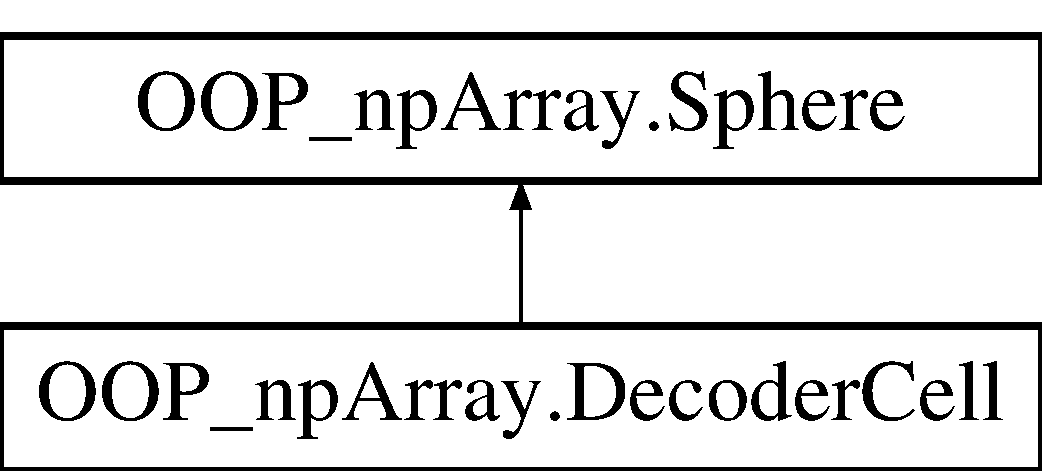
\includegraphics[height=2.000000cm]{class_o_o_p__np_array_1_1_decoder_cell}
\end{center}
\end{figure}
\subsection*{Public Member Functions}
\begin{DoxyCompactItemize}
\item 
\mbox{\Hypertarget{class_o_o_p__np_array_1_1_decoder_cell_af7cfba9c006d9b79594cebd2d583dd99}\label{class_o_o_p__np_array_1_1_decoder_cell_af7cfba9c006d9b79594cebd2d583dd99}} 
def {\bfseries \+\_\+\+\_\+init\+\_\+\+\_\+} (self, args)
\item 
def \mbox{\hyperlink{class_o_o_p__np_array_1_1_decoder_cell_a91863318471abedb0cd6db43b22a4ece}{express\+Lectins}} (self, lectin\+\_\+list, density\+\_\+percentage)
\begin{DoxyCompactList}\small\item\em Method to attach \mbox{\hyperlink{class_o_o_p__np_array_1_1_lectin}{Lectin}} objects to \mbox{\hyperlink{class_o_o_p__np_array_1_1_decoder_cell}{Decoder\+Cell}} objects. \end{DoxyCompactList}\end{DoxyCompactItemize}
\subsection*{Public Attributes}
\begin{DoxyCompactItemize}
\item 
\mbox{\Hypertarget{class_o_o_p__np_array_1_1_decoder_cell_a8cb11c80902e372d0ebc6540acdf5c51}\label{class_o_o_p__np_array_1_1_decoder_cell_a8cb11c80902e372d0ebc6540acdf5c51}} 
{\bfseries lectin\+\_\+density}
\item 
\mbox{\Hypertarget{class_o_o_p__np_array_1_1_decoder_cell_ab5afb370eb7adc4f6e2e6e6d9e73c7e6}\label{class_o_o_p__np_array_1_1_decoder_cell_ab5afb370eb7adc4f6e2e6e6d9e73c7e6}} 
{\bfseries lectin}
\end{DoxyCompactItemize}


\subsection{Detailed Description}
\mbox{\hyperlink{class_o_o_p__np_array_1_1_decoder_cell}{Decoder\+Cell}} is a subclass of \mbox{\hyperlink{class_o_o_p__np_array_1_1_sphere}{Sphere}} and represents immune cells (such as T\+H\+P-\/1 cells) that express Lectins which bind to \mbox{\hyperlink{class_o_o_p__np_array_1_1_glycan}{Glycan}} structures and engage in immune response by secreting cytokines. 

\subsection{Member Function Documentation}
\mbox{\Hypertarget{class_o_o_p__np_array_1_1_decoder_cell_a91863318471abedb0cd6db43b22a4ece}\label{class_o_o_p__np_array_1_1_decoder_cell_a91863318471abedb0cd6db43b22a4ece}} 
\index{O\+O\+P\+\_\+np\+Array\+::\+Decoder\+Cell@{O\+O\+P\+\_\+np\+Array\+::\+Decoder\+Cell}!express\+Lectins@{express\+Lectins}}
\index{express\+Lectins@{express\+Lectins}!O\+O\+P\+\_\+np\+Array\+::\+Decoder\+Cell@{O\+O\+P\+\_\+np\+Array\+::\+Decoder\+Cell}}
\subsubsection{\texorpdfstring{express\+Lectins()}{expressLectins()}}
{\footnotesize\ttfamily def O\+O\+P\+\_\+np\+Array.\+Decoder\+Cell.\+express\+Lectins (\begin{DoxyParamCaption}\item[{}]{self,  }\item[{}]{lectin\+\_\+list,  }\item[{}]{density\+\_\+percentage }\end{DoxyParamCaption})}



Method to attach \mbox{\hyperlink{class_o_o_p__np_array_1_1_lectin}{Lectin}} objects to \mbox{\hyperlink{class_o_o_p__np_array_1_1_decoder_cell}{Decoder\+Cell}} objects. 

Every \mbox{\hyperlink{class_o_o_p__np_array_1_1_decoder_cell}{Decoder\+Cell}} objects contains one type of \mbox{\hyperlink{class_o_o_p__np_array_1_1_lectin}{Lectin}} with a given density. Parameter lectins\+\_\+list is handed over to the constructor of \mbox{\hyperlink{class_o_o_p__np_array_1_1_lectin}{Lectin}}.


\begin{DoxyParams}[1]{Parameters}
\mbox{\tt in}  & {\em lectin\+\_\+list} & see documentation for class \mbox{\hyperlink{class_o_o_p__np_array_1_1_lectin}{Lectin}}. \\
\hline
\end{DoxyParams}


The documentation for this class was generated from the following file\+:\begin{DoxyCompactItemize}
\item 
O\+O\+P\+\_\+np\+Array.\+py\end{DoxyCompactItemize}

\hypertarget{class_o_o_p__np_array_1_1_glycan}{}\section{O\+O\+P\+\_\+np\+Array.\+Glycan Class Reference}
\label{class_o_o_p__np_array_1_1_glycan}\index{O\+O\+P\+\_\+np\+Array.\+Glycan@{O\+O\+P\+\_\+np\+Array.\+Glycan}}


Objects of the class \mbox{\hyperlink{class_o_o_p__np_array_1_1_glycan}{Glycan}} are attached to objects of the class \mbox{\hyperlink{class_o_o_p__np_array_1_1_bead}{Bead}}.  


\subsection*{Public Member Functions}
\begin{DoxyCompactItemize}
\item 
\mbox{\Hypertarget{class_o_o_p__np_array_1_1_glycan_a6ef0d3f7150be4d292bd1f0839b1db04}\label{class_o_o_p__np_array_1_1_glycan_a6ef0d3f7150be4d292bd1f0839b1db04}} 
def {\bfseries \+\_\+\+\_\+init\+\_\+\+\_\+} (self, glycan\+\_\+names\+\_\+list, glycan\+\_\+types\+\_\+list)
\end{DoxyCompactItemize}
\subsection*{Public Attributes}
\begin{DoxyCompactItemize}
\item 
\mbox{\Hypertarget{class_o_o_p__np_array_1_1_glycan_a05a9a4f3e2f75c16c74c2af9a5f965c3}\label{class_o_o_p__np_array_1_1_glycan_a05a9a4f3e2f75c16c74c2af9a5f965c3}} 
{\bfseries name}
\item 
\mbox{\Hypertarget{class_o_o_p__np_array_1_1_glycan_a3cd19a1f38e8ee9d84235ef9b0a86310}\label{class_o_o_p__np_array_1_1_glycan_a3cd19a1f38e8ee9d84235ef9b0a86310}} 
{\bfseries type}
\end{DoxyCompactItemize}


\subsection{Detailed Description}
Objects of the class \mbox{\hyperlink{class_o_o_p__np_array_1_1_glycan}{Glycan}} are attached to objects of the class \mbox{\hyperlink{class_o_o_p__np_array_1_1_bead}{Bead}}. 

They represent glycan structures which are divided into different types.


\begin{DoxyParams}[1]{Parameters}
\mbox{\tt in}  & {\em glycan\+\_\+names\+\_\+list} & List of Strings containing the \char`\"{}real\char`\"{} names of \mbox{\hyperlink{class_o_o_p__np_array_1_1_glycan}{Glycan}} structures to be added to the \mbox{\hyperlink{class_o_o_p__np_array_1_1_bead}{Bead}}. List may contain any number of members, including 0 \\
\hline
\mbox{\tt in}  & {\em glycan\+\_\+types\+\_\+list} & List of Strings containing the respective types of \mbox{\hyperlink{class_o_o_p__np_array_1_1_glycan}{Glycan}} structures. These types determine the outcome of the interaction between \mbox{\hyperlink{class_o_o_p__np_array_1_1_bead}{Bead}} and \mbox{\hyperlink{class_o_o_p__np_array_1_1_decoder_cell}{Decoder\+Cell}} as specified in the cytokine dictionary. If the this list does not contain the same number of member as glycan\+\_\+names\+\_\+list, the program terminates. \\
\hline
\end{DoxyParams}


The documentation for this class was generated from the following file\+:\begin{DoxyCompactItemize}
\item 
O\+O\+P\+\_\+np\+Array.\+py\end{DoxyCompactItemize}

\hypertarget{class_o_o_p__np_array_1_1_lectin}{}\section{O\+O\+P\+\_\+np\+Array.\+Lectin Class Reference}
\label{class_o_o_p__np_array_1_1_lectin}\index{O\+O\+P\+\_\+np\+Array.\+Lectin@{O\+O\+P\+\_\+np\+Array.\+Lectin}}


Objects of the class \mbox{\hyperlink{class_o_o_p__np_array_1_1_lectin}{Lectin}} are attached to objects of the class \mbox{\hyperlink{class_o_o_p__np_array_1_1_decoder_cell}{Decoder\+Cell}}.  


\subsection*{Public Member Functions}
\begin{DoxyCompactItemize}
\item 
\mbox{\Hypertarget{class_o_o_p__np_array_1_1_lectin_a6c63531d83a862fa9d3b089354a26f86}\label{class_o_o_p__np_array_1_1_lectin_a6c63531d83a862fa9d3b089354a26f86}} 
def {\bfseries \+\_\+\+\_\+init\+\_\+\+\_\+} (self, lectin\+\_\+list)
\end{DoxyCompactItemize}
\subsection*{Public Attributes}
\begin{DoxyCompactItemize}
\item 
\mbox{\Hypertarget{class_o_o_p__np_array_1_1_lectin_aedbfd75de0d5fcd2cda6bf05efc329ca}\label{class_o_o_p__np_array_1_1_lectin_aedbfd75de0d5fcd2cda6bf05efc329ca}} 
{\bfseries name}
\end{DoxyCompactItemize}


\subsection{Detailed Description}
Objects of the class \mbox{\hyperlink{class_o_o_p__np_array_1_1_lectin}{Lectin}} are attached to objects of the class \mbox{\hyperlink{class_o_o_p__np_array_1_1_decoder_cell}{Decoder\+Cell}}. 

They represent lectin receptors which recognize certain sets of glycans on other cells, beads, viruses a.\+s.\+o.


\begin{DoxyParams}[1]{Parameters}
\mbox{\tt in}  & {\em lectin\+\_\+list} & List of Strings containing the names of \mbox{\hyperlink{class_o_o_p__np_array_1_1_lectin}{Lectin}} receptors to be added to the \mbox{\hyperlink{class_o_o_p__np_array_1_1_decoder_cell}{Decoder\+Cell}}. These names appear in the dictionary. List may contain any number of members, including 0. \\
\hline
\end{DoxyParams}


The documentation for this class was generated from the following file\+:\begin{DoxyCompactItemize}
\item 
O\+O\+P\+\_\+np\+Array.\+py\end{DoxyCompactItemize}

\hypertarget{class_o_o_p__np_array_1_1_simulation}{}\section{O\+O\+P\+\_\+np\+Array.\+Simulation Class Reference}
\label{class_o_o_p__np_array_1_1_simulation}\index{O\+O\+P\+\_\+np\+Array.\+Simulation@{O\+O\+P\+\_\+np\+Array.\+Simulation}}


Dictionary is based on Geijtenbeek \& Gringhuis C-\/type lectin receptors in the control of T helper cell differentiation Nature Reviews Immunology volume 16, pages 433–448 (2016)  




\subsection{Detailed Description}
Dictionary is based on Geijtenbeek \& Gringhuis C-\/type lectin receptors in the control of T helper cell differentiation Nature Reviews Immunology volume 16, pages 433–448 (2016) 

The documentation for this class was generated from the following file\+:\begin{DoxyCompactItemize}
\item 
O\+O\+P\+\_\+np\+Array.\+py\end{DoxyCompactItemize}

\hypertarget{class_o_o_p__np_array_1_1_sphere}{}\section{O\+O\+P\+\_\+np\+Array.\+Sphere Class Reference}
\label{class_o_o_p__np_array_1_1_sphere}\index{O\+O\+P\+\_\+np\+Array.\+Sphere@{O\+O\+P\+\_\+np\+Array.\+Sphere}}


\mbox{\hyperlink{class_o_o_p__np_array_1_1_sphere}{Sphere}} serves as superclass for the two spherical objects indroduced below.  


Inheritance diagram for O\+O\+P\+\_\+np\+Array.\+Sphere\+:\begin{figure}[H]
\begin{center}
\leavevmode
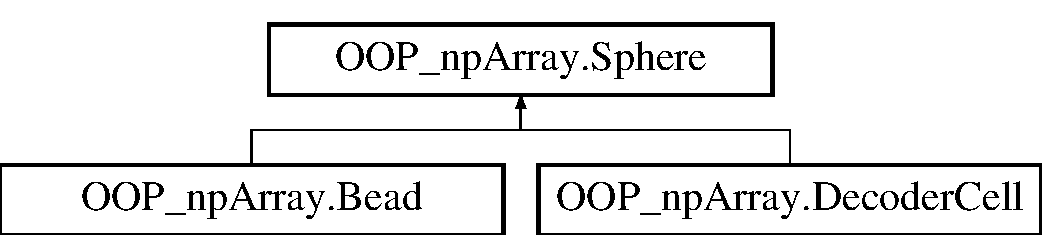
\includegraphics[height=2.000000cm]{class_o_o_p__np_array_1_1_sphere}
\end{center}
\end{figure}
\subsection*{Public Member Functions}
\begin{DoxyCompactItemize}
\item 
\mbox{\Hypertarget{class_o_o_p__np_array_1_1_sphere_a5885b15f6bcd60c64ddb557e21dbff3f}\label{class_o_o_p__np_array_1_1_sphere_a5885b15f6bcd60c64ddb557e21dbff3f}} 
def {\bfseries \+\_\+\+\_\+init\+\_\+\+\_\+} (self, I\+D\+\_\+string)
\end{DoxyCompactItemize}
\subsection*{Public Attributes}
\begin{DoxyCompactItemize}
\item 
\mbox{\Hypertarget{class_o_o_p__np_array_1_1_sphere_ab9142543fa0581404e28c131cc5b8541}\label{class_o_o_p__np_array_1_1_sphere_ab9142543fa0581404e28c131cc5b8541}} 
{\bfseries ID}
\item 
\mbox{\Hypertarget{class_o_o_p__np_array_1_1_sphere_a27390f074435cb70bdfa9f3f4495270f}\label{class_o_o_p__np_array_1_1_sphere_a27390f074435cb70bdfa9f3f4495270f}} 
{\bfseries coordinates}
\end{DoxyCompactItemize}


\subsection{Detailed Description}
\mbox{\hyperlink{class_o_o_p__np_array_1_1_sphere}{Sphere}} serves as superclass for the two spherical objects indroduced below. 


\begin{DoxyParams}[1]{Parameters}
\mbox{\tt in}  & {\em ID} & Identifier \\
\hline
 & {\em coordinates} & Empty. Will be filled when added to \mbox{\hyperlink{class_o_o_p__np_array_1_1_well}{Well}}. \\
\hline
\end{DoxyParams}


The documentation for this class was generated from the following file\+:\begin{DoxyCompactItemize}
\item 
O\+O\+P\+\_\+np\+Array.\+py\end{DoxyCompactItemize}

\hypertarget{class_o_o_p__np_array_1_1_well}{}\section{O\+O\+P\+\_\+np\+Array.\+Well Class Reference}
\label{class_o_o_p__np_array_1_1_well}\index{O\+O\+P\+\_\+np\+Array.\+Well@{O\+O\+P\+\_\+np\+Array.\+Well}}


The class \mbox{\hyperlink{class_o_o_p__np_array_1_1_well}{Well}} describes the sample, in which binding events take place.  


Inheritance diagram for O\+O\+P\+\_\+np\+Array.\+Well\+:\begin{figure}[H]
\begin{center}
\leavevmode
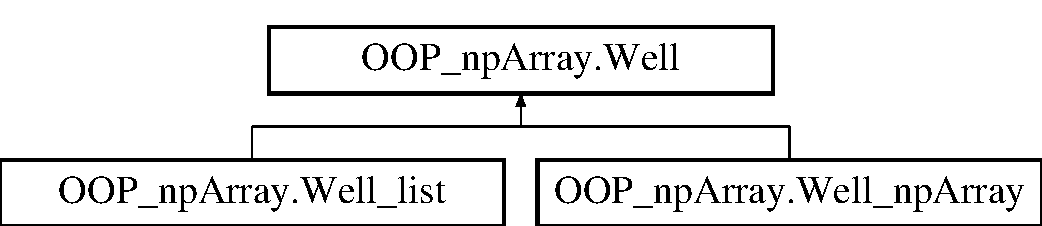
\includegraphics[height=2.000000cm]{class_o_o_p__np_array_1_1_well}
\end{center}
\end{figure}
\subsection*{Public Member Functions}
\begin{DoxyCompactItemize}
\item 
\mbox{\Hypertarget{class_o_o_p__np_array_1_1_well_ab7cb865616e6fd3e6e98604400329f0c}\label{class_o_o_p__np_array_1_1_well_ab7cb865616e6fd3e6e98604400329f0c}} 
def {\bfseries \+\_\+\+\_\+init\+\_\+\+\_\+} (self, x, y, z)
\item 
def \mbox{\hyperlink{class_o_o_p__np_array_1_1_well_a8991b9d19614962be6a088031f780554}{border\+Control}} (self, coordinates, dx, dy, dz)
\begin{DoxyCompactList}\small\item\em The method border\+Control ensures that objects\textquotesingle{} coordinates don\textquotesingle{}t exceed the well\textquotesingle{}s size. \end{DoxyCompactList}\end{DoxyCompactItemize}
\subsection*{Public Attributes}
\begin{DoxyCompactItemize}
\item 
\mbox{\Hypertarget{class_o_o_p__np_array_1_1_well_a7ef6da8f1d375133df8edff40ef3d48d}\label{class_o_o_p__np_array_1_1_well_a7ef6da8f1d375133df8edff40ef3d48d}} 
{\bfseries size}
\end{DoxyCompactItemize}


\subsection{Detailed Description}
The class \mbox{\hyperlink{class_o_o_p__np_array_1_1_well}{Well}} describes the sample, in which binding events take place. 

It serves a a superclass for two subclasses of which one uses Num\+Py Arrays as a container for onjects of the classes \mbox{\hyperlink{class_o_o_p__np_array_1_1_bead}{Bead}} and \mbox{\hyperlink{class_o_o_p__np_array_1_1_decoder_cell}{Decoder\+Cell}} while the other one uses built-\/in Python lists for this purpose.


\begin{DoxyParams}[1]{Parameters}
\mbox{\tt in}  & {\em \mbox{[}x,y,z\mbox{]}} & Size of the well. \\
\hline
\end{DoxyParams}


\subsection{Member Function Documentation}
\mbox{\Hypertarget{class_o_o_p__np_array_1_1_well_a8991b9d19614962be6a088031f780554}\label{class_o_o_p__np_array_1_1_well_a8991b9d19614962be6a088031f780554}} 
\index{O\+O\+P\+\_\+np\+Array\+::\+Well@{O\+O\+P\+\_\+np\+Array\+::\+Well}!border\+Control@{border\+Control}}
\index{border\+Control@{border\+Control}!O\+O\+P\+\_\+np\+Array\+::\+Well@{O\+O\+P\+\_\+np\+Array\+::\+Well}}
\subsubsection{\texorpdfstring{border\+Control()}{borderControl()}}
{\footnotesize\ttfamily def O\+O\+P\+\_\+np\+Array.\+Well.\+border\+Control (\begin{DoxyParamCaption}\item[{}]{self,  }\item[{}]{coordinates,  }\item[{}]{dx,  }\item[{}]{dy,  }\item[{}]{dz }\end{DoxyParamCaption})}



The method border\+Control ensures that objects\textquotesingle{} coordinates don\textquotesingle{}t exceed the well\textquotesingle{}s size. 

If a step in random\+Walk would lead to a forbidden value, the respective step value will be set to 0 and the object won\textquotesingle{}t move this turn as if repelled from the well\textquotesingle{}s borders.


\begin{DoxyParams}[1]{Parameters}
\mbox{\tt in}  & {\em coordinates} & The object\textquotesingle{}s coordinates before the move. \\
\hline
\mbox{\tt in}  & {\em dx,dy,dz} & The randomly chosen next steps. \\
\hline
\mbox{\tt out}  & {\em dx,dy,dz} & The \\
\hline
\end{DoxyParams}


The documentation for this class was generated from the following file\+:\begin{DoxyCompactItemize}
\item 
O\+O\+P\+\_\+np\+Array.\+py\end{DoxyCompactItemize}

\hypertarget{class_o_o_p__np_array_1_1_well__list}{}\section{O\+O\+P\+\_\+np\+Array.\+Well\+\_\+list Class Reference}
\label{class_o_o_p__np_array_1_1_well__list}\index{O\+O\+P\+\_\+np\+Array.\+Well\+\_\+list@{O\+O\+P\+\_\+np\+Array.\+Well\+\_\+list}}


Subclass of \mbox{\hyperlink{class_o_o_p__np_array_1_1_well}{Well}} using built-\/in python lists as containers for objects of the classes \mbox{\hyperlink{class_o_o_p__np_array_1_1_bead}{Bead}} and \mbox{\hyperlink{class_o_o_p__np_array_1_1_decoder_cell}{Decoder\+Cell}}.  


Inheritance diagram for O\+O\+P\+\_\+np\+Array.\+Well\+\_\+list\+:\begin{figure}[H]
\begin{center}
\leavevmode
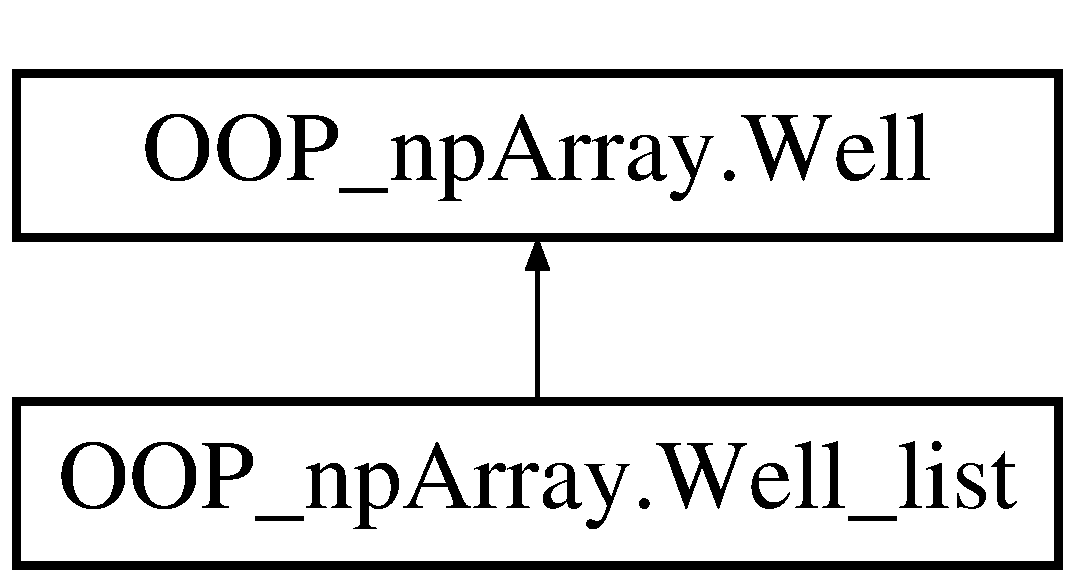
\includegraphics[height=2.000000cm]{class_o_o_p__np_array_1_1_well__list}
\end{center}
\end{figure}
\subsection*{Public Member Functions}
\begin{DoxyCompactItemize}
\item 
\mbox{\Hypertarget{class_o_o_p__np_array_1_1_well__list_a34452e04bc0aa035ca3049b2a4cbe5bd}\label{class_o_o_p__np_array_1_1_well__list_a34452e04bc0aa035ca3049b2a4cbe5bd}} 
def {\bfseries \+\_\+\+\_\+init\+\_\+\+\_\+} (self, x, y, z, n\+\_\+beads, n\+\_\+cells)
\item 
def \mbox{\hyperlink{class_o_o_p__np_array_1_1_well__list_ae0961c99dd36f4417bc5c7f3cfe81b67}{add\+Bead}} (self, i, bead, glyan\+\_\+name\+\_\+string, glycan\+\_\+type\+\_\+string, density\+\_\+percentage)
\begin{DoxyCompactList}\small\item\em Method to add objects of class \mbox{\hyperlink{class_o_o_p__np_array_1_1_bead}{Bead}} to the bead list. \end{DoxyCompactList}\item 
\mbox{\Hypertarget{class_o_o_p__np_array_1_1_well__list_a4faff6c708781f38124239448043117c}\label{class_o_o_p__np_array_1_1_well__list_a4faff6c708781f38124239448043117c}} 
def {\bfseries add\+Decoder\+Cell} (self, i, decoder\+Cell, lectin\+\_\+name\+\_\+string, lectin\+\_\+type\+\_\+string)
\end{DoxyCompactItemize}
\subsection*{Public Attributes}
\begin{DoxyCompactItemize}
\item 
\mbox{\Hypertarget{class_o_o_p__np_array_1_1_well__list_a04f23430cc3154d47b51bfe2b12e8bfb}\label{class_o_o_p__np_array_1_1_well__list_a04f23430cc3154d47b51bfe2b12e8bfb}} 
{\bfseries size}
\item 
\mbox{\Hypertarget{class_o_o_p__np_array_1_1_well__list_a5155967229f404a247799167c5c637a5}\label{class_o_o_p__np_array_1_1_well__list_a5155967229f404a247799167c5c637a5}} 
{\bfseries beads}
\item 
\mbox{\Hypertarget{class_o_o_p__np_array_1_1_well__list_ab5516771f8d44ae1c00b78abf101d5a6}\label{class_o_o_p__np_array_1_1_well__list_ab5516771f8d44ae1c00b78abf101d5a6}} 
{\bfseries decoder\+Cells}
\end{DoxyCompactItemize}


\subsection{Detailed Description}
Subclass of \mbox{\hyperlink{class_o_o_p__np_array_1_1_well}{Well}} using built-\/in python lists as containers for objects of the classes \mbox{\hyperlink{class_o_o_p__np_array_1_1_bead}{Bead}} and \mbox{\hyperlink{class_o_o_p__np_array_1_1_decoder_cell}{Decoder\+Cell}}. 

\subsection{Member Function Documentation}
\mbox{\Hypertarget{class_o_o_p__np_array_1_1_well__list_ae0961c99dd36f4417bc5c7f3cfe81b67}\label{class_o_o_p__np_array_1_1_well__list_ae0961c99dd36f4417bc5c7f3cfe81b67}} 
\index{O\+O\+P\+\_\+np\+Array\+::\+Well\+\_\+list@{O\+O\+P\+\_\+np\+Array\+::\+Well\+\_\+list}!add\+Bead@{add\+Bead}}
\index{add\+Bead@{add\+Bead}!O\+O\+P\+\_\+np\+Array\+::\+Well\+\_\+list@{O\+O\+P\+\_\+np\+Array\+::\+Well\+\_\+list}}
\subsubsection{\texorpdfstring{add\+Bead()}{addBead()}}
{\footnotesize\ttfamily def O\+O\+P\+\_\+np\+Array.\+Well\+\_\+list.\+add\+Bead (\begin{DoxyParamCaption}\item[{}]{self,  }\item[{}]{i,  }\item[{}]{bead,  }\item[{}]{glyan\+\_\+name\+\_\+string,  }\item[{}]{glycan\+\_\+type\+\_\+string,  }\item[{}]{density\+\_\+percentage }\end{DoxyParamCaption})}



Method to add objects of class \mbox{\hyperlink{class_o_o_p__np_array_1_1_bead}{Bead}} to the bead list. 

Coordinates of the \mbox{\hyperlink{class_o_o_p__np_array_1_1_bead}{Bead}} are randomly chosen between 0 and size of the \mbox{\hyperlink{class_o_o_p__np_array_1_1_well}{Well}} in the respective dimension.


\begin{DoxyParams}[1]{Parameters}
\mbox{\tt in}  & {\em i} & Not used here, but neccessary for convenient switching between container types. \\
\hline
\mbox{\tt in}  & {\em bead} & Object of class \mbox{\hyperlink{class_o_o_p__np_array_1_1_bead}{Bead}} to be added. \\
\hline
\mbox{\tt in}  & {\em } & \\
\hline
\end{DoxyParams}


The documentation for this class was generated from the following file\+:\begin{DoxyCompactItemize}
\item 
O\+O\+P\+\_\+np\+Array.\+py\end{DoxyCompactItemize}

\hypertarget{class_o_o_p__np_array_1_1_well__np_array}{}\section{O\+O\+P\+\_\+np\+Array.\+Well\+\_\+np\+Array Class Reference}
\label{class_o_o_p__np_array_1_1_well__np_array}\index{O\+O\+P\+\_\+np\+Array.\+Well\+\_\+np\+Array@{O\+O\+P\+\_\+np\+Array.\+Well\+\_\+np\+Array}}
Inheritance diagram for O\+O\+P\+\_\+np\+Array.\+Well\+\_\+np\+Array\+:\begin{figure}[H]
\begin{center}
\leavevmode
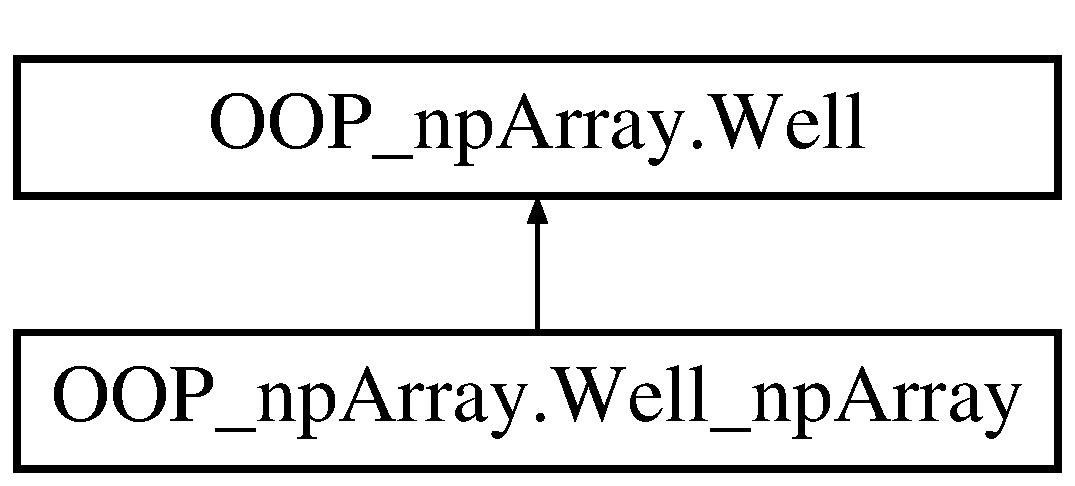
\includegraphics[height=2.000000cm]{class_o_o_p__np_array_1_1_well__np_array}
\end{center}
\end{figure}
\subsection*{Public Member Functions}
\begin{DoxyCompactItemize}
\item 
\mbox{\Hypertarget{class_o_o_p__np_array_1_1_well__np_array_a444855f0c55c0420a6ef5d5c0ac3214a}\label{class_o_o_p__np_array_1_1_well__np_array_a444855f0c55c0420a6ef5d5c0ac3214a}} 
def {\bfseries \+\_\+\+\_\+init\+\_\+\+\_\+} (self, x, y, z, n\+\_\+beads, n\+\_\+cells)
\item 
\mbox{\Hypertarget{class_o_o_p__np_array_1_1_well__np_array_a2a7090962b7123e4400fa3343e0c1289}\label{class_o_o_p__np_array_1_1_well__np_array_a2a7090962b7123e4400fa3343e0c1289}} 
def {\bfseries add\+Bead} (self, i, bead, glyan\+\_\+name\+\_\+string, glycan\+\_\+type\+\_\+string, density\+\_\+percentage)
\item 
\mbox{\Hypertarget{class_o_o_p__np_array_1_1_well__np_array_a736fded2de7a8996ddceb86a38ee6fa4}\label{class_o_o_p__np_array_1_1_well__np_array_a736fded2de7a8996ddceb86a38ee6fa4}} 
def {\bfseries add\+Decoder\+Cell} (self, i, decoder\+Cell, lectin\+\_\+name\+\_\+string, lectin\+\_\+type\+\_\+string)
\end{DoxyCompactItemize}
\subsection*{Public Attributes}
\begin{DoxyCompactItemize}
\item 
\mbox{\Hypertarget{class_o_o_p__np_array_1_1_well__np_array_a9a8c256bed5cd50e3e5670c1f8d430a2}\label{class_o_o_p__np_array_1_1_well__np_array_a9a8c256bed5cd50e3e5670c1f8d430a2}} 
{\bfseries beads}
\item 
\mbox{\Hypertarget{class_o_o_p__np_array_1_1_well__np_array_ab6c127c23c6e613f7d32242742970a2f}\label{class_o_o_p__np_array_1_1_well__np_array_ab6c127c23c6e613f7d32242742970a2f}} 
{\bfseries decoder\+Cells}
\end{DoxyCompactItemize}


The documentation for this class was generated from the following file\+:\begin{DoxyCompactItemize}
\item 
O\+O\+P\+\_\+np\+Array.\+py\end{DoxyCompactItemize}

%--- End generated contents ---

% Index
\backmatter
\newpage
\phantomsection
\clearemptydoublepage
\addcontentsline{toc}{chapter}{Index}
\printindex

\end{document}
